%kate: default-dictionary en;

\documentclass[eprint]{actapoly}

\usepackage{graphicx,adjustbox}
\usepackage{algorithm}
\usepackage{algpseudocode}
\usepackage{amssymb}
\usepackage{tikz}
\usepackage{tikzscale}
\usetikzlibrary{matrix,shapes,arrows,positioning,chains,calc}
%\usepackage{amsmath, amssymb, amsfonts, amsthm}
%\usepackage{float}
%\usepackage{graphicx}
\usepackage{subcaption}
\floatstyle{plaintop}
\restylefloat{table}

\hyphenpenalty=100000

%\usepackage{draftwatermark}
%\SetWatermarkText{DRAFT}
%\SetWatermarkScale{1}
%\SetWatermarkLightness{0.9}

\begin{document}

%\title[Example of an Article with a Long Title]
%{Example of an Article with a Long Title, the Title Should Be Capitalised 
%Properly in the Code Long Long}
\title[Trajectory Generation Approach]
{Multi-Robot Motion Planning: a Modified Receding Horizon Approach for reaching Goal States}

\author[J. M. Mendes Filho]{Jos\'{e} M. Mendes Filho}{my,their}
\correspondingauthor[E. Lucet]{Eric Lucet}{my}{eric.lucet@cea.fr}

\institution{my}{CEA, LIST, Interactive Robotics Laboratory, Gif-sur-Yvette, 
F-91191, France}
\institution{their}{ENSTA
Paristech,
Unité
d'Informatique et
d'Ingénierie 
des Systèmes,
828 bd des Marechaux, 91762, France}
%\institution{their}{ENSTA Paristech, Unit\'{e} informatique et Ingénierie des 
%Système, 828 boulevard des Marechaux, F-91762, France}
%\institution{their}{CEA, LIST, Interactive Robotics Laboratory, 
%Gif-sur-Yvette, F-91191, France}

\begin{abstract}

%This paper proposes the real-time implementation of a multi-robot optimal collision-free motion planner algorithm based on a receding horizon approach, for the navigation of a team of mobile robots evolving in an industrial context in presence of different structures of obstacles. The method is validated in simulation environment for a team of three robots. Then, impact of the algorithm parameters setting is studied with regard to critical performance criteria, being mainly real-time implementation, obstacle avoidance and time to complete the task.

This paper proposes the real-time implementation of an algorithm for collision-free motion planning based on a receding horizon approach, for the navigation of a team of mobile robots in presence of obstacles of different shapes. The method is simulated with three robots. Impact of parameters is studied with regard to computation time, obstacle avoidance and travel time.

% In view 
 
\end{abstract}

\keywords{\mbox{multi-robot motion planning}, \mbox{nonholonomic mobile robot}, \mbox{distributed planning}, \mbox{receding horizon}}

\maketitle




\section{Introduction}\label{sec:intro}




%General Context


The %command and
control of mobile robots is a long-standing subject of research 
in the robotics domain. A trending application of mobile robotic systems
is their use in industrial supply-chains for processing orders and optimizing products' storage and distribution. Companies such as Amazon and the logistic provider IDEA Groupe employ mobile multi-robot systems (Kiva systems, Scallog respectively) for autonomously processing client orders~\cite{Gizmag,supplychain}.
%such as teams of autonomous forklift trucks
%(for instance Kiva robots used by Amazon~\cite{Gizmag},
%to improve their commercial performance,
Such logistics tasks became increasingly complex as sources of uncertainty, such as human presence, are admitted in the work environment.

%Problem

One basic requirement for such mobile multi-robot systems is the capacity of motion planning, that is, generating admissible configuration and input trajectories connecting two arbitrary states. For solving the motion planning problem, different 
constraints must be taken into account, in particular, the robot's kinematic and geometric constraints.
%
%\begin{itemize}
%
% \item robot's kinematic and dynamic constraints;
%
% \item geometric constraints;

% \item constraints associated with uncertainties about the current state of 
%world and the outcome of actions.

%\end{itemize}

The first constraints derive directly from the mobile robot architecture 
implying, in particular, in nonholonomic constraints.
Geometric constraints result from the need of preventing the robot to assume
specific configurations
in order to avoid collisions, communication lost, etc.
% the impossibility of the robots to assume some specific 
%configurations  due to the presence of obstacles, environment bounds, communication range, etc. 
%In turn, uncertainty constraints come from the impossibility of the robots to have an 
%absolute and complete perception of the world (including theirs own states) as 
%well as the outcome of non-stochastic events.


We are particularly interested in solving the problem of planning a 
trajectory for a team of nonholonomic mobile robots, in a partially known 
environment occupied by static obstacles, being efficient with respect to the 
travel time (amount of time to go from initial to goal configuration).


%State of Art

A great amount of work towards collision-free motion 
planning for cooperative multi-robot systems has been proposed. That work can
be split into centralized and distributed approaches.
Centralized approaches are usually formulated as an optimal
control problem that takes all robots in the team into account at once.
This produces solutions closer to the optimal one than distributed approaches. However, the computation time, security vulnerability and communication 
requirements can make it impracticable, specially for a great number of 
robots~\cite{Borrelli2006}.

Distributed methods based in probabilistic~\cite{Sanchez2002} and artificial 
potential fields~\cite{Khatib1986} approaches, for instance, are computationally fast.
However, they deal with collision avoidance as a cost function to be minimized.
But rather than having a cost that increases as paths leading
to collision are considered, collision avoidance should to be considered as hard constraints of the problem.


Other distributed algorithms are based on receding horizon approaches.
In \cite{Defoort2009} a brief comparison of the main distributed receding 
methods is made as well as the presentation of the base approach extended in
our work.
In this approach each robot optimizes only its own 
trajectory at each computation/update horizon. In order to
avoid robot-to-robot collisions and lost of communication, neighbor robots 
exchange information about their intended trajectories before 
performing the update. Intended trajectories are computed by each robot
ignoring constraints that take the other robots into account.

Identified drawbacks of this approach are the dependence on 
several parameters for achieving real-time performance and good solution 
optimality, the difficulty to adapt it for handling dynamic obstacles, the 
impossibility of bringing the robots to a precise goal state and the limited
geometric representation of obstacles.

%Some work has been done towards analytic methods for solving the problem for 
%certain classes of systems (~\cite{})
%TODO cite
%. However~\cite{Schwartz1988} shows 
%that analytic methods  are inapplicable for nonholonomic systems in presence of 
%obstacles.
%
%
%Cell decomposition methods, as presented in~\cite{Latombe1991}, have the 
%downside of requiring a structured configuration space and an \textit{a priori} 
%model of its connectivity. Besides, the cell decomposition reduces the space 
%of admissible solutions.
%
% 
%
%Initially proposed in~\cite{Khatib1986}, the vector field obstacle avoidance 
%method was improved along time for treating problems such as oscillation of the 
%solution for narrow passages. This method does not present a near optimal 
%generated trajectory.
%
% 
%
%Elastic band approach initially proposed by~\cite{Quinlan1994} and extended to 
%mobile manipulators in~\cite{Brock et Khatib, 1998} uses approximations of the 
%trajectory shape (combinations of arcs and straight lines) limiting the space 
%of solutions and thus making this method inappropriate for really constrained 
%environments.
%
% 
%
%The dynamic window approach~\cite{Fox1997} can handle trajectory 
%planning for robots at high speeds and in presence of obstacles. But it is not 
%flexible enough to be extended to a multi-robot system.

 

%What do we propose

Therefore, in this paper, we propose a motion planning algorithm that extends 
the approach presented in~\cite{Defoort2009}. In this modified algorithm goal states can be precisely reached and more complexes forms of obstacles handled.
Furthermore, we perform an investigation 
about how the method's parameters impact a set of performance criteria.
Thus, this distributed algorithm is able to find collision-free trajectories and 
computes the corresponding angular and longitudinal velocities for a multi-robot system in 
presence of static obstacles perceived by the robots as they evolve in their environment.

%This algorithm finds collision-free trajectories and computes the corresponding
%angular and longitudinal velocities for a multi-robot system in 
%presence of static obstacles perceived by the robots as they evolve 
%in their environment. The dynamic trajectories computed are near optimal with 
%respect to the total time spent going from the initial configuration to the 
%final one. Besides, this algorithm uses a distributed approach making the 
%system more robust to communication outages and individual robot failure than 
%compared to a centralized approach. Identified drawbacks are the dependence on 
%several parameters for achieving real-time performance and good solution 
%optimality, and the difficulty of handling dynamic obstacles as it is.

%This algorithm is an extension of the work done in~\cite{Defoort2007a}. In particular,
%improvements are proposed for the respect of a precise final configuration of the 
%multi-robot system. Also, investigation about how to set parameters for achieving
%satisfying solutions was performed.

%solving the nonlinear 
%programming problem (NLP).

 

%Plan

This paper is structured as follows. The second section states the problem to
be resolved, pointing out the cost function for motion planning and all constraints
that need to be respected by the computed solution.
%motion planning algorithm that solves the problem of one robot going from an initial 
%configuration to a final one in the presence of static obstacles.
The third section explains the algorithm for resolving the motion planning problem and gives
some remarks on how to resolve the constrained optimization problems associated
with the method.
%section extends the method presented in the second section so a collision-free 
%trajectory that maintains the communication link between the robots in the 
%team can be computed.
The forth section is dedicated to the results found using
this method and the analysis of the specific performance criteria and 
how they are impacted by the algorithm parameters.
%In the fifth section this
%approach is compared to another one presented in~\cite{Kelly_2003}.
Finally, in last section we present our conclusions and perspectives.

%\newpage
%\mbox{}\newpage

\section{Problem Statement}\label{sec:problem}

%We consider the following assumptions for the simulation of our approach:
\subsection{Assumptions}
In the development of the approach presented in this paper, the following assumptions are made:

\begin{enumerate}

    \item The motion of the multi-robot system begins at
    the instant $t_{init}$ and goes until the instant $t_{final}$.

    \item The team of robots consists of a set $\mathcal{R}$ of $B$
    nonholonomic mobile robots.
    
    \item A robot (denoted $R_b,\ R_b \in \mathcal{R},\ b \in \{0,\dots,B-1\}$) is 
    geometrically represented by a circle of radius $\rho_b$ centered at
    $(x_b, y_b)$.
        
    \item All obstacles in the environment are considered static. They can be
    represented by a set $\mathcal{O}$ of $M$ static obstacles.
    
    \item An obstacle (denoted $O_m,\ $\mbox{$O_m \in \mathcal{O}$}$,\ $
    \mbox{$m \in \{0,\ \dots, M-1\}$}) is geometrically represented either as
    a circle or as a convex polygon. In the case of a circle its radius is
    denoted $r_{O_m}$ centered at $(x_{O_m},y_{O_m})$.
    
    \item For a given instant $t_k \in [t_{init},\ t_{final}]$, any obstacle
    $O_m$ is considered detected by the robot $R_b$ whenever the distance between
    their geometric centers is less than or equal to the detection radius $d_{b,sen}$
    of the robot $R_b$.
    Therefore, this obstacle $O_m$ is part of the set $\mathcal{O}_b$
    ($\mathcal{O}_b \subset \mathcal{O}$) of detected obstacles.
    
    \item A robot has precise knowledge of the position and geometric 
    representation of a detected obstacle, i.e., obstacles perception issues
    are neglected.
    
    \item A robot can access 
    information about any robot in the team by using 
    a wireless communication link. Latency, communication outages and other
    problems associated
    to the that communication link are neglected.
        
    \item The dynamic model of the multi-robot systems is neglected.
    
    \item The input (or control) vector of a mobile robot $R_b$ is bounded.
    
%    \item The motion planner in a robot $R_b$ (with $n \in {0,\dots,B-1}$) has
%    access to the following information:
%    \begin{enumerate}
%        \item current and past configuration of the robot $R_b$;
%        \item $R_b$'s goal configuration;
%        \item $R_b$'s input limits;
%        \item The map function to pass from flat space to state and input space and
%        its inverse;
%        \item  
%    \end{enumerate}

%     as well as the its robot's goal configuration, the input limits,
%    its kinematic
%    model and bijective mapping function for passing from the flat space to the
%    actual state and input spaces;
%    
%    \item Each robot have sensors that can detect the surrounding region within a
%    radius $\rho_d$. Any object having its geometric center within this region is
%    considered detect by the robot;

\end{enumerate}

\subsection{Constraints and cost functions}

After giving the assumptions in the previous Subsection,
we can define the constraints and the cost function for the
multi-robot navigation.

\begin{enumerate}

    \item The solution of the motion planning problem
    for the robot $R_b$ represented by the pair
    $(q^{*}_b(t), u^{*}_b(t))$ --
    $q^{*}_b(t) \in \mathbb{R}^n$ being the solution trajectory for
    the robot's configuration and $u^{*}_b(t) \in \mathbb{R}^p$ the solution
    trajectory for the robot's input -- must satisfy the
    robots kinematic model equation:
%    For a robot $R_b$     
%    its kinematic model equation
%    must hold for a computed solution to the
%    motion planning problem:
    \begin{equation}\label{eq:kinematic}
        \dot{q}^{*}_b(t) = f(q^{*}_b(t),u^{*}_b(t)),\quad \forall t \in [t_{init}, t_{final}].
    \end{equation}
    where \mbox{$f\,:\,\mathbb{R}^{n}\times \mathbb{R}^{p}\rightarrow \mathbb{R}^n$} the
	is the vector-valued function modeling the robot kinematics.
%	with $q^{*}_b(t) \in \mathbb{R}^n$ the solution 
%	trajectory for the robot's configuration,
%	$u^{*}_b(t) \in \mathbb{R}^p$ the solution trajectory
%	for the robot's input and
%	
    
    \item The planned initial configuration and initial 
    input for the robot $R_b$ must
    be equal to the initial configuration and initial
    input of $R_b$:
    \begin{equation}
        q^{*}_{b}(t_{init}) = q_{b,init},
    \end{equation}
    \begin{equation}
        u^{*}_{b}(t_{init}) = u_{b,init}.
    \end{equation}

    \item The planned final configuration and final 
    input for the robot $R_b$ must
    be equal to the goal configuration and goal
    input for $R_b$:
    \begin{equation}\label{eq:finalconfig}
        q^{*}_{b}(t_{final}) = q_{b,goal},
    \end{equation}
    \begin{equation}\label{eq:finalinput}
        u^{*}_{b}(t_{final}) = u_{b,goal}.
    \end{equation}

    \item Practical limitations of the input impose
    the following constraint: $\forall t \in [t_{init}, t_{final}]$, $\forall i \in [1,2,\cdots, p]$,
    \begin{equation}
        |u^{*}_{b,i}(t)| \leq u_{b,i,max}.
    \end{equation}
    
    \item The cost for the multi-robot system navigation is defined as:
    \begin{equation}
        L(q(t),u(t)) = \sum_{b=0}^{B-1}L_b(q_b(t), u_b(t), q_{b,goal},u_{b,goal})
    \end{equation}
    where $L_b(q_b(t), u_b(t), q_{b,goal},u_{b,goal})$ is the 
    integrated cost for one robot
    motion planning (see~\cite{Defoort2009}).
    
    \item 
    %TODO define the functions "distance" robot-to-obstacle:
    To ensure collision avoidance with obstacles, the euclidean 
    distance between
    a robot and an obstacle (denoted $\mathrm{d}(R_b, O_m)\ |\ O_m
    \in \mathcal{O}_b, R_b \in \mathcal{B} $) has to satisfy:
    \begin{equation}
    	\mathrm{d}(R_b, O_m) \geq 0.
    \end{equation}
    
    For the circle representation of an obstacle the distance
    $\mathrm{d}(R_b, O_m)$ is defined as:
    \begin{equation*}
        \sqrt{(x_{b} - x_{O_m})^2 + (y_{b} - y_{\mathrm{O}_m})^2}  - \rho_b - r_{O_m}.
    \end{equation*}
    
    For the convex polygon representation, the distance was calculated
    using three different
    definitions, according to the Voronoi region~\cite{ericson2004real}
    $R_b$ is located.
%    Voronoi regions are 
%    defined by
%    the lines containing the sides ($s$ lines) and by the lines passing
%    through the vertexes that are orthogonal to the sides ($r$ lines) of
%    the convex polygon. 
%    Figure~\ref{fig:convexpolygon} shows an
%    quadrilateral $ABCD$ representation of an obstacle where three of the nine
%    regions were distinguished. 
%
%
%    %Each of these three region are 
%%     For a generic convex polygon three different
%%    kinds of regions can be defined. 
%    
%%    One kind is defined by the two lines passing 
%%    through a vertix, another by one line passing through two consecutive vertese
%%     Figure~\ref{fig:convexpolygon} shows an
%%    quadrilateral $ABCD$ representation of the obstacle where three of the nine . For this
%%    representation three different kinds of regions can be define.
%    
%    
%%    regions he three kinds
%%    of regions for a quadrilateral $ABCD$ representation.    
%    
%%	In this example, the region in which the robot $R_b$ is located
%%	at an instant $t_k$
%%	can be computed by evaluating the line
%% 	equations 
%% 	$s_{AB}$, $s_{BC}$, $s_{CD}$, $s_{DA}$, $r_{AB}$, $r_{AD}$, $r_{BA}$, $r_{BA}$,
%% 	$r_{BC}$, $r_{BA}$, $r_{BC}$, $r_{CB}$, $r_{CD}$, $r_{DC}$ and $r_{DA}$ for 
%% 	the position associated with the configuration $q^*_b(t_k)$.
% 	
%%    The region which the position associated with a given configuration $q_b$
%%    is in can be computed as follows.
%    
%    For these three regions, the distance
%    robot-to-quadrilateral is computed as follows:
%    \begin{enumerate}
%    
%	   	\item \label{it:vora} If robot in region $1$:
%   	   	\begin{equation*}
%    	    \sqrt{(x_{b} - x_{A})^2 + (y_{b} - y_{A})^2} - \rho_b
%	    \end{equation*}
%	    which is simply the distance of the robot to the vertex $A$.
%	    
%	    \item \label{it:vorb} If robot in region $2$:	    
%		\begin{equation*}
%			\mathrm{d}(s_{DA}, (x_{b}, y_{b})) - \rho_b
%		\end{equation*}
%		where
%   	   	\begin{equation*}
%    	    \mathrm{d}(s_{DA}, (x_{b}, y_{b})) =\\ \frac{|a_{s_{DA}}x_{b} + b_{s_{DA}}y_{b}
%    	    + c_{s_{DA}}|}{\sqrt{a_{s_{DA}}^2 + b_{s_{DA}}^2}}.
%	    \end{equation*}
%	    
%	    The distance $\mathrm{d}(s_{DA}, (x_{b}, y_{b}))$ represents the distance
%	    from the robot to the side $DA$.
%	    
%	    \item If robot in region $3$:
%   	   	\begin{equation*}
%    	    -\min\left(\mathrm{d}(s_{AB}, (x_{b}, y_{b})), \cdots, \mathrm{d}(s_{DA}, (x_{b}, y_{b}))\right) - \rho_b
%	    \end{equation*}
%	    which represents the amount of penetration of the robot in the obstacle.
%	    
%    \end{enumerate}
%    
%    The distance computation for other regions can be easily 
%    inferred from equations in items~\ref{it:vora} and~\ref{it:vorb}.
%    
%    \begin{figure}[!h]
%	\centering
%	{
%	    \begin{tikzpicture}
%		[polygon/.style={very thick, black},
%		axis/.style={-,blue,thick},
%		point/.style={very thick,black},
%		afill/.style = {fill=blue!20,fill opacity=0.5},
%		bfill/.style = {fill=red!20,fill opacity=0.5}]
%		
%		\fill[afill] (0,1,0) -- (-0.5,3,0) -- (-1.5,3,0) -- (-1.5,-.5,0) --cycle;
%		\fill[bfill] (0,1,0) -- (4,2,0) -- (3.75,3.,0) -- (-0.5,3,0) --cycle;
%		
%		\draw[axis] (-.25,2.,0) -- (.5,-1.,0) node[anchor=west,color=blue]
%		{$r_{AD}$}; % y = 1. - 4.x
%		
%		\draw[axis] (1.,2.,0) -- (-1.,0.,0) node[anchor=west,color=blue]
%		{$r_{AB}$};%y = x+1
%	
%		\draw[axis] (3.75,3.,0) -- (4.375,0.5,0) node[anchor=west,color=blue]
%		{$r_{DA}$}; %y = 18.-4. x
%	
%		\draw[axis,red] (-1.,.75,0) -- (5.,2.25,0) node[anchor=north,color=red]
%		{$s_{DA}$};
%		
%		\draw[polygon,fill=gray!50] (0,1,0)  -- (1,0,0) node[below] {$B$}
%		-- (3,0,0) node[below] {$C$} -- (4,2,0) -- cycle;
%		\node[text width=0cm] at (-0.4,1.2,0) {$A$};
%		\node[text width=0cm] at (4.1,2.3,0) {$D$};
%			
%		\draw[point] (2.0,2.4,0) node[anchor=east]{\textbullet $2$};
%		\draw[point] (-0.5,1.5,0) node[anchor=east]{\textbullet $1$};
%		\draw[point] (2.6,0.5,0) node[anchor=east]{\textbullet $3$};
%	
%		\end{tikzpicture}}
%	\caption{Voronoi regions used for case differentiation. \label{fig:convexpolygon}}
%	\end{figure}

    \item 
    In order to prevent inter-robot collisions, the following constraint must be satisfied:
    $\forall\ (R_b, R_c) \in \mathcal{R} \times \mathcal{R}, b\neq c, c \in \mathcal{C}_b$,
    %o a robot $R_b$ avoid collision with other robots the following
    %relation must be satisfied. 
%    In order to avoid inter-robot collision the following constraint
%    must be respect by the robots $R_b$ and $R_b$:
    \begin{equation}\label{eq:coll}
	    \mathrm{d}(R_b,R_c) - \rho_b -\rho_c \geq 0
    \end{equation}
    where $\mathrm{d}(R_b,R_c) = \sqrt{(x_{b} - x_{c})^2 + (y_{b} - y_{c})^2}$ and
    $\mathcal{C}_b$ is the set of robots that present a collision risk with
    $R_b$.
%    This constraint justifies the need for a communication link between the robots.
    
    \item Finally, the need of a communication link between two robots $(R_b, R_c)$ yields to
    the following constraint:
    %In addition, for a given pair of robots $R_b R_c$ that must keep
    %a communication link between them the following equation 
    \begin{equation}\label{eq:com}
    	\mathrm{d}(R_b,R_c)  - \min(d_{b,com}, d_{c,com}) \leq 0
    \end{equation}
    with $d_{b,com}, d_{c,com}$ the communication link reach of each robot and
    $\mathcal{D}_b$ is the set of robots that present a communication lost risk with
    $R_b$.
\end{enumerate}
%\newpage
%\mbox{}\newpage



\section{Distributed motion planning}



\subsection{Receding horizon approach}\label{subsec:rha}

%Defoort give in \cite{    Defoort2007a} an example showing how a unicycle model 
%can be written using the flatness property.
%The basis algorithm for planning for a mono robot is based on the optimization 
%problem shown in (\ref{eq:}) and (\ref{eq:}).
%TODO present method or make reference to Defoort introducing $T_c$, $T_p$ etc.

Since the environment is progressively perceived by the robots and new obstacles may 
appear as time passes,
planning the whole motion from initial to goal configurations before the beginning
of the motion is
not a satisfying approach. Planning locally and replanning is 
more suitable for taking new information, as they come, into account. Besides, the computation cost of finding a motion plan using
the first approach may be prohibited high if the planning complexity depends
on the distance between start and goal configurations.

Therefore, an on-line motion planner 
%that computes the configuration and input 
%trajectories as the multi-robot system evolves in the environment
is proposed.
In order to do so a receding horizon control approach~\cite{Keviczky2006} is used.

Two fundamental concepts of this approach are the planning horizon $T_p$ and 
update/computation horizon $T_c$. $T_p$ is the timespan for which a solution 
will be computed and
$T_c$ is the time horizon during which a plan is executed while the
next plan, for the next timespan $T_p$, is being computed.
The problem of producing a motion plan during a $T_c$ time interval is called
here a receding horizon planning problem.

For each receding horizon planning problem, the following steps are performed:
\paragraph{Step 1.}\label{step1} All robots in the team compute an intended solution trajectory (denoted $(\hat{q}_b(t), \hat{u}_b(t))$)
by solving a constrained optimization problem. Coupling
constraints (\ref{eq:coll}) and (\ref{eq:com}) that involve 
other robots in the team are ignored.
\paragraph{Step 2.}\label{step2} Robots involved in a potential conflict (that is, risk of collision 
or lost of communication) update their trajectories computed during \nameref{step1} by solving another constrained optimization problem
that additionally takes into account
coupling constraints (\ref{eq:coll}) and (\ref{eq:com}).
This is done by using the other robots' intended
trajectories computed in the previous step as an estimate of those robots'
final trajectories. If a robot is not involved in any conflict, \nameref{step2}
is not executed and its final
solution trajectory is identical to the one estimated in \nameref{step1}.

\mbox{}

All robots in the team use the same $T_p$ and $T_c$ for assuring synchronization when exchanging information about their positions and intended trajectories.

For each of these steps and for each robot in the team, one constrained optimization problem is resolved. The cost function to be minimized in those
optimization problems
%, proposed in \cite{Defoort2007a}
is the geodesic distance of a robot's current configuration to its goal configuration.
This assures that the robots are driven towards their goal.

This two step scheme is explained in details in~\cite{Defoort2009, Defoort2007a} where 
constrained optimization problems associated to the receding horizon 
optimization problem are formulated.

However, constraints related to the goal configuration and goal input of the motion planning problem are
neglected in their method.
Constraints (\ref{eq:finalconfig}) and (\ref{eq:finalinput}) are left out of the planning.
For taking them into account, a termination procedure is proposed in the following that enables the robots to reach their goal state.



\subsection{Motion planning termination}



%As the robots evolve in the environment using the distributed receding horizon planning, their configuration approximate to the goal configuration.
%%That is so because the  since the distance between current and final state is what is to 
%%be minimized.
%But simply stopping the motion planner when robots are in the neighborhood 
%of their final configuration leaves 
%constraints~\ref{eq:finalconfig} and~\ref{eq:finalinput} unsatisfied.

%Furthermore, the use of a constant planning horizon $T_p$ prevents the robot of
%finding 

After stopping the receding horizon planning algorithm, we propose a 
termination planning that considers those constraints related to
the goal state.
%in the \textbf{termination optimization problem}
This enables the robots to reach their goal states.

%The constraints associated to the final configuration and input have to be integrated 
%into the optimization problem. In addition, the timespan for performing this last
%termination plan cannot be constant and must be one of the values to be calculated.
%The fixed planning horizon has to be made variable in order to get to the 

The criterion used to pass from the receding 
horizon planning to the termination planning is based on the distance between
goal and current position of the robots. It is defined by the equation~\ref{eq:stopcond}:
\begin{align}\label{eq:stopcond}
  d_{rem} \geq d_{min} + T_c \cdot v_{max}
\end{align}
This condition ensures that the termination plan will be planned for at least a 
$d_{min}$ distance from the robot's goal position.
This minimal distance is assumed to be sufficient for the robot to reach the 
goal configuration.

Before solving the termination planning problem new parameters for 
the solution representation and computation are calculated by taking into
account the estimate remaining distance and the typical distance traveled
for a $T_p$ planning horizon.
%(as better explained in TODO REF).
This is done in order to rescale the configuration intended for a previous 
planning horizon not necessarily equal to the new one. Potentially, this
rescaling will decrease the computation time for the termination planning.

The following pseudo code~\ref{cod:algo} summarizes the planning algorithm    
and the Figure~\ref{fig:recedinghor} illustrates how plans would be generated
through time by the algorithm.

In the pseudo code, we see the call of a {\scshape PlanSec} procedure.
It corresponds to the resolution of the receding horizon planning 
problem as defined in subsection~\ref{subsec:rha}.

{\scshape PlanLastSec} is the procedure solving the termination planning
problem. This problem is similar to the receding horizon planning problems.

%TODO

It also has the two steps presented before for computing an intended plan and
for updating it, if need be, so conflicts are avoided.

%TODO

The difference consists in how the optimization problems associated to it are 
defined. The optimization problem defined in (\ref{eq:costsa}) and
(\ref{eq:constsa}) is the problem solved at the first step.
%(denoted ($\hat{q}_b(t)$, $\hat{u}_b(t)$))
The optimization
problem associated with the second step is defined (\ref{eq:cost}) and (\ref{eq:const}).
Besides, in both new constrained optimal problems, the planning horizon is not
a fixed constant as before, instead it is a part of the solution to be found.

Then, for generating the intended plan the following is resolved:
\begin{align}\label{eq:costsa}
\underset{\hat{q}_b(t),\hat{u}_b(t),T_f}{\mathrm{min}} L_{b,f}(\hat{q}_b(t), \hat{u}_b(t), q_{b,goal},u_{b,goal})
\end{align}
under the following constraints for $\tau_k = kT_c$ with $k$ the number of receding horizon
problems solved before the termination problem:
\begin{equation}\label{eq:constsa}
\left\lbrace\begin{array}{lcl}
    \dot{\hat{q}}_b(t) = f(\hat{q}_b(t),\hat{u}_b(t)),\ \ \forall t \in [\tau_{k}, \tau_{k}+T_f]\\
    \hat{q}_b(\tau_{k}) = q^*_{b}(\tau_{k-1}+T_c)\\
    \hat{u}_b(\tau_{k}) = u^*_{b}(\tau_{k-1}+T_c)\\
    \hat{q}_b(\tau_{k}+T_f) = q_{b,goal}\\
    \hat{u}_b(\tau_{k}+T_f) = u_{b,goal}\\
    |\hat{u}_{b,i}(t)| \leq u_{b,i,max},\ \ \forall i \in [1,p],\forall t \in (\tau_{k}, \tau_{k}+T_f)\\
    d(R_b, O_m) \geq 0,\quad \forall O_m \in \mathcal{O}_b, t \in (\tau_{k}, \tau_{k}+T_f)
\end{array}\right.
\end{equation}

And for generating the final solution:
\begin{align}\label{eq:cost}
\underset{q^*_b(t),u^*_b(t),T_f}{\mathrm{min}} L_{b,f}(q^*_b(t), u^*_b(t), q_{b,goal},u_{b,goal})
\end{align}
under the following constraints:
\begin{equation}\label{eq:const}
\left\lbrace\begin{array}{lcl}
    \dot{q^*}_b(t) = f(q^*_b(t),u^*_b(t)),\ \ \forall t \in [\tau_{k}, \tau_{k}+T_f]\\
    q^*_b(\tau_{k}) = q^*_{b}(\tau_{k-1}+T_c)\\
    u^*_b(\tau_{k}) = u^*_{b}(\tau_{k-1}+T_c)\\
    q^*_b(\tau_{k}+T_f) = q_{b,goal}\\
    u^*_b(\tau_{k}+T_f) = u_{b,goal}\\
    |u^*_{b,i}(t)| \leq u_{b,i,max},\ \ \forall i \in [1,p],\forall t \in (\tau_{k}, \tau_{k}+T_f)\\
    d(R_b, O_m) \geq 0,\ \ \forall O_m \in \mathcal{O}_b, \forall t \in (\tau_{k}, \tau_{k}+T_f)\\
    \mathrm{d}(R_b, R_c) - \rho_b - \rho_c \geq 0,\ \ \forall R_c \in \mathcal{C}_b, \forall t \in (\tau_{k}, \tau_{k}+T_f)\\
    \mathrm{d}(R_b, R_d) - \min(d_{b,com},d_{d,com}) \geq 0,\ \ \forall R_d \in \mathcal{D}_b,\\
    \quad \quad \quad \quad \quad \quad \quad \quad \quad \quad \quad \quad \quad \quad \quad \forall t \in (\tau_{k}, \tau_{k}+T_f)\\
    \mathrm{d}(q^*_b(t), \hat{q}_b(t)) \leq \xi,\ \ \forall t \in (\tau_{k}, \tau_{k}+T_f)
\end{array}\right.
\end{equation}

A possible definition for the $L_{b,f}$ cost function present in the equations above can be simply $T_f$.
The sets $\mathcal{O}_b$, $\mathcal{C}_b$ and $\mathcal{D}_b$ are functions of
$\tau_k$.

\begin{algorithm}
    \caption{Motion planning algorithm\label{cod:algo}}
    \label{swpa}
    \begin{algorithmic}[1] % The number tells where the line numbering should start
        \Procedure{Plan}{} %\Comment{The g.c.d. of a and b}
%	    \State $knots \gets $\Call{GenKnots}{$t_p,d_{spl},n_{knots}$}
%	    \State $time \gets $\Call{LineSpacing}{$0,t_p,n_{s}$}
	    %\State $z_{latest} \gets $\Call{$\varphi_0$}{$q_{initial}$}
	    \State $q_{latest} \gets q_{initial}$
	    %\State $ctrlpts \gets $\Call {InitCtrlPts}{$q_{initial},q_{final},T_p,u_{max}$}
	    %\State \Call{Init}{}
	    \State $d_{rem} \gets |${\scshape Pos}$(q_{final}) - ${\scshape Pos}$(q_{latest})|$
	    \While{$d_{rem} \geq d_{min} + T_c \cdot v_{max}$}
	    \State \Call{InitSolRepresentation}{$\cdots$}
		\State $q_{latest} \gets $\Call{PlanSec}{$\cdots$}
		\State $d_{rem} \gets |${\scshape Pos}$(q_{final}) - ${\scshape Pos}$(q_{latest})|$
		
	    \EndWhile\label{planningwhile}
	    \State \Call{RescaleRepresentation}{$\cdots$}
%	    \State $s \gets $\Call {Min}{$\tfrac{d_{rem}}{v_{max}\cdot t_p}, 1.0$}
%	    \State $n_{knots} \gets $\Call{Max}{\Call{Round}{$s\cdot n_{knots}$}$, d_{spl}$}
%	    \State $n_{s} \gets $\Ca1ll {Max}{\Call{Round}{$s\cdot n_{s}$}$, n_{knots} + d_{spl}$}
	    \State $T_f \gets $\Call{PlanLastSec}{$\cdots$}
	    
%            \State $r\gets a \bmod b$
%            \While{$r\not=0$} %\Comment{We have the answer if r is 0
%                \State $a \gets b$
%                \State $b \gets r$
%                \State $r \gets a \bmod b$
%            \EndWhile\label{euclidendwhile}
%            \State \textbf{return} $b$%\Comment{The gcd is b}
        \EndProcedure
    \end{algorithmic}
\end{algorithm}

\begin{figure}[!h]
  \centering
  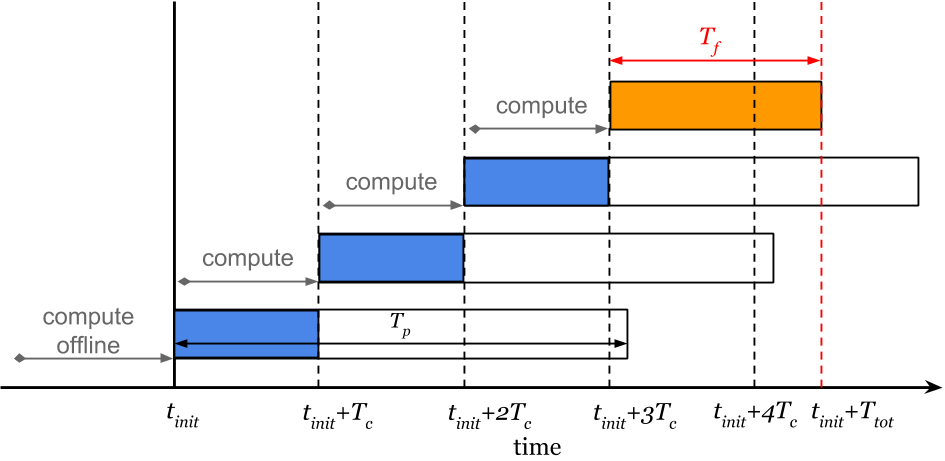
\includegraphics[width=\linewidth]{./images/receding_horizon/recedinghorizon2.png} %
  %\rule{5cm}{5cm} % <-- this is just a black box substitute for graphics
  \caption{Receding horizon scheme with termination plan. The timespan $T_f$ represents the duration of the plan for reaching the goal configuration.\label{fig:recedinghor}}
\end{figure}


% Define block styles
%\tikzset{
%desicion/.style={
%    diamond,
%    draw,
%    aspect=1.8,
%    text width=7em,
%    text badly centered,
%    inner sep=0pt
%},
%block/.style={
%    rectangle,
%    draw,
%    text width=10em,
%    text centered,
%    rounded corners
%},
%cloud/.style={
%    draw,
%    ellipse,
%    minimum height=2em
%},
%descr/.style={
%    fill=white,
%    inner sep=2.5pt
%},
%connector/.style={
%    -latex,
%    font=\scriptsize
%},
%rectangle connector/.style={
%    connector,
%    to path={(\tikztostart) -- ++(#1,0pt) \tikztonodes |- (\tikztotarget) },
%    pos=0.5
%},
%rectangle connector/.default=-2cm,
%straight connector/.style={
%    connector,
%    to path=--(\tikztotarget) \tikztonodes
%}
%}
%
%\begin{figure}[H]
%\begin{adjustbox}{max width=\linewidth}
%    \begin{tikzpicture}
%		\matrix (m)[matrix of nodes, column  sep=1cm,row  sep=8mm, align=center, nodes={rectangle,draw, anchor=center} ]{
%		    |[block]| {Start} &  & \\
%		    |[block]| {Initilize} &  & \\
%		    |[block]| {Update}     & |[desicion]| {Neighborhood of $q_{b,goal}$ reached? (eq:~\ref{eq:stopcond})} &      |[block]| {Update} \\
%		    |[block]| {Solve $NLP_{b,1}(\tau_k)$} & &  |[block]| {Rescale} \\
%		    |[block]| {Computation of conflict sets $\mathcal{C}_{b,com}$ and $\mathcal{C}_{b,coll}$}     &  &         |[block]| {Solve $NLP_{b,3}(\tau_k)$}\\
%		    |[desicion]| {Is $\mathcal{C}_{b,com}(\tau_k) \bigcup \mathcal{C}_{b,coll}(\tau_k)$ empty?} &  &|[block]| {Computation of conflict sets $\mathcal{C}_{b,com}$ and $\mathcal{C}_{b,coll}$}\\
%		    |[block]| {Sync with $\forall R_c | R_c \in \mathcal{C}_{b,com} \bigcup \mathcal{C}_{b,coll}$}& & |[desicion]| {Is $\mathcal{C}_{b,com}(\tau_k) \bigcup \mathcal{C}_{b,coll}(\tau_k)$ empty?}\\
%		    |[block]| {Exchange intented trajectories with $\forall R_c | R_c \in \mathcal{C}_{b,com} \bigcup \mathcal{C}_{b,coll}$}     & &   |[block]| {Sync with $\forall R_c | R_c \in \mathcal{C}_{b,com} \bigcup \mathcal{C}_{b,coll}$}\\
%		    |[block]| {Solve $NLP_{b,2}(\tau_k)$}     & |[block]| {Wait while $t-\tau_{ref}<T_c$} &    |[block]| {Exchange intented trajectories with $\forall R_c | R_c \in \mathcal{C}_{b,com} \bigcup \mathcal{C}_{b,coll}$} \\
%		     & |[block]| {Finish}  &  |[block]| {Solve $NLP_{b,4}(\tau_k)$}\\
%		};
%		
%		
%		\path let \p1=(m-7-3) in coordinate (invis) at (2.5,\y1);
%		\path let \p1=(m-10-3) in coordinate (invis2) at (2.5,\y1);
%		
%		\path let \p1=(m-6-1) in coordinate (invis1) at (-2.5,\y1);
%		\path let \p1=(m-9-2) in coordinate (invis12) at (-2.5,\y1);
%		
%		\path [>=latex,->] (m-1-1) edge (m-2-1);
%		\path [>=latex,->] (m-2-1) edge node[anchor=west, near start] {$q^*_{b}(\tau_{-1}+T_c) \leftarrow q_{init}, \dots$} (m-3-1);
%		\path [>=latex,->] (m-3-1) edge node[anchor=west, near start] {$\mathcal{O}_n(\tau_k), \tau_{ref} \leftarrow t$} (m-4-1);
%		\path [>=latex,->] (m-4-1) edge (m-5-1);
%		\path [>=latex,->] (m-5-1) edge (m-6-1);
%		\path [>=latex,->] (m-6-1) edge node[anchor=east] {no} (m-7-1);
%		\path [>=latex,->] (m-6-1) edge node[anchor=north] {yes} (invis1);
%		\path [>=latex,->] (invis1) edge (invis12);
%		%\path [>=latex,->,bend left] (m-6-1) edge node[anchor=east] {yes} (m-9-2);
%		\path [>=latex,->] (m-7-1) edge (m-8-1);
%		\path [>=latex,->] (m-8-1) edge (m-9-1);
%		\path [>=latex,->] (m-9-1) edge (m-9-2);
%		\path [>=latex,->] (m-9-2) edge (m-3-2);
%		\path [>=latex,->] (m-3-2) edge node[anchor=north] {no} (m-3-1);
%		\path [>=latex,->] (m-3-2) edge node[anchor=north] {yes} (m-3-3);
%		\path [>=latex,->] (m-3-3) edge node[anchor=west, near start] {$\mathcal{O}_n(\tau_k), \tau_{ref} \leftarrow t$} (m-4-3);
%		\path [>=latex,->] (m-4-3) edge (m-5-3);
%		\path [>=latex,->] (m-5-3) edge (m-6-3);
%		\path [>=latex,->] (m-6-3) edge (m-7-3);
%		\path [>=latex,->] (m-7-3) edge node[anchor=north] {yes} (invis);
%		\path [>=latex,->] (invis) edge (invis2);
%		\path [>=latex,->] (m-7-3) edge node[anchor=east] {no}  (m-8-3);
%		\path [>=latex,->] (m-8-3) edge (m-9-3);
%		\path [>=latex,->] (m-9-3) edge (m-10-3);
%		\path [>=latex,->] (m-10-3) edge (m-10-2);
%		\node[blue!80,text width=10cm] at ($(m-9-1.south east) + (0.0,-1.7)$){Receding Horizon Planning};
%		\draw[blue!80,line width=1.0pt,dotted] ($(m-3-1.north west)+(-0.4,1.2)$)  rectangle ($(m-9-2.south east)+(0.2,-0.6)$);
%		
%		\end{tikzpicture}
%		\end{adjustbox}
%    \caption{Flowchart illustrating the distributed local motion planning\label{fig:flowchart}}
%\end{figure}

\subsection{Strategies for solving the constrained optimization problems}



\subsubsection{Flatness property}

As explained in~\cite{Defoort2007a}, all mobile robots consisting of a solid
block in motion can be modeled as a flat system. 
This means that a change of variables is possible in a way that states and
inputs of the kinematic model of the mobile robot can be written in terms
of a new variable, called flat output ($z$), and its $l$th first derivatives.
The value of $l\ |\ l \leq n$ depends on the kinematic model of the mobile robot.
Therefore, the flat output can completely determine behavior of the system.

%\begin{figure}[!h]\centering
%  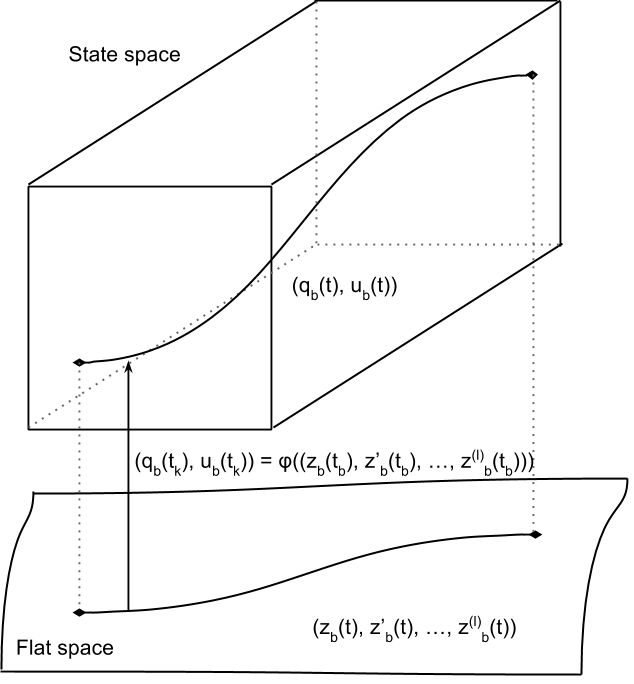
\includegraphics[width=.7\linewidth]{./images/flatness.png} %
%  \caption{Flatness\label{fig:flatness}}
%\label{fig:res}
%\end{figure}

Searching for a solution to our problem in the flat space rather than in
the actual configuration space of the system presents advantages.
It prevents the need for integrating the differential equations
of system (constraint ~\ref{eq:kinematic}) and reduces the dimension of the 
problem of finding an optimal admissible trajectory.
%($l<n$, $n$ being the configuration vector dimension).
After finding (optimal) trajectories in the flat space, it is possible
to retrieve back the original configuration and input trajectories.
%as shown in Figure~\ref{fig:flatness}.

\subsubsection{Parametrization of the flat output by B-splines}

Another important aspect of this approach is the parametrization of 
the flat output trajectory. As done in~\cite{Milam2003}, the use
of B-spline functions present interesting properties.
\begin{itemize}


 \item It is possible to specify a level of continuity $C^k$ when using
 B-splines without additional constraints.
 
 \item B-spline presents a local support -- changes in parameters values have a 
 local impact on the resulting curve.
 
 
\end{itemize}
The first property is very well suited for parametrizing the flat output since
its $l$th first derivatives will be needed when computing the system actual state
and input trajectories. The second property is important when searching for an
admissible solution in the flat space; such parametrization is more efficient
and well-conditioned than, for instance, a polynomial parametrization \cite{Milam2003}.

%As said before $l$ derives from the kinematic model of the robot.

This choice for parameterizing the flat output introduces a new parameter to be set in
the motion planning algorithm which is the number of non-null knots intervals 
(denoted simply $N_{knots}$). This parameter plus the $l$ value determines how many 
control points will be used for generating the B-splines.

\subsubsection{Optimization solver}

%There exists a variety of numerical optimization packages implemented in many different %programming languages available for solving optimization problems~\cite{pyopt-paper}.

The optimization problems associated with finding the solution $q^*(t), u^*(t)$
are solved using a numerical optimization solver. For all time dependent constraints time sampling is used. This introduces
a new parameter in the algorithm: the time sampling for optimization $N_s$.
Each constraint that must be satisfied $\forall t \in (\tau_k, \tau_k + T_f)$ implies in $N_s$ equations.

The need of a solver that supports nonlinear equality and inequality constrains
restricts the number of numerical optimization solvers to be considered.

For our initial implementation of the motion planning algorithm, the
SLSQP optimizer stood out
as a good option. Besides being able to handle nonlinear equality and inequality 
constrains, its availability in the minimization module of the open-source
scientific package Scipy~\cite{Scipy} helps to facilitate the motion planner implementation.
%Finally, when compared with others free licensed optimizers such as the ones
%available in the Python-based package PyOpt, SLSQP showed fast and better
%results.

However, an error was experienced using this optimizer which uses the SLSQP 
Optimization subroutine originally implemented by Dieter Kraft~\cite{Kraft1988}.
As the cost function value becomes too high (typically for values greater than 
$10^3$), the optimization algorithm finishes with the "Positive 
directional derivative for linesearch" error message. This appears to be
a numerical stability problem experienced by other users as discussed in~\cite{slsqperror}.

For working around this problem, we proposed a change in the objective functions
of the receding horizon optimization problems. This change aims to keep the 
evaluated cost of the objective function around a known value when close to the optimal
solution instead of having a cost depending on the goal configuration (which can be arbitrarily distant from the current position).

We simply exchanged the goal position point in the cost function by a new point computed as follows:
$$
    p_{b,new} = \frac{p_{b,goal} - p_{b}(\tau_{s-1}+T_c) }{\mathrm{norm}(p_{b,goal} - p_{b}(\tau_{s-1}+T_c) )} \alpha T_pv_{b,max}
$$
Where $p_{b,goal}$ and $p_{b}(\tau_{s-1}+T_c)$ are the positions associated with configurations $q_{b,goal}$ and $q_{b}(\tau_{s-1}+T_c)$ respectively, $\alpha\ |\ 
\alpha \geq 1, \alpha \in \mathbb{R}$ is a constant for controlling how far from the
current position the new point is placed, the product $T_pv_{b,max}$ the maximum possible distance covered by $R_b$ during a planning horizon and $s\ |\ s \in [0, k), s \in \mathbb{N}$ the current receding horizon problem index.

%The impacts of these parameters on the solution quality and computation time are discussed in the following section.

%change of assuming a high value when converging to a solution. Instead of %computing the distance 
%between the final position of a plan $T_p$ A change in the cost function

%Other two algorithms from another Python-based optimization package, PyOpt 
%\cite{pyopt-paper} were tested with 

%As explained in~\ref{Defoort2009}, a Feasible Sequential Quadratic Programming 
%is best suited for solving the motion
%planning problem as stated in thins paper. 
%This class of solvers compute at every iteration solution
%that respects the problem constraints.

%TODO keep explaining, present SLSQL and ALGENCAN, present reasons why we used 
%SLSQP (i.e. availability in python, free license, and faster then ALGENCAN)

%\newpage
%\mbox{}\newpage



\section{Simulation results}




Results and their analysis for the motion planner presented in the previous sections are 
presented here.

The trajectory and velocities shown in Figures~\ref{fig:collision} and~\ref{fig:nocollision}
illustrate a motion planning solution found for a team of three robots.
They plan their motion in an environment where three static obstacles are present.
Each point along the trajectory line of a robot represents the beginning
of a $Tc$ update/computation horizon.

It is possible to see on those figures how the planner generates configuration and 
input trajectories satisfying the constraints associated with the goal states.

In particular, in Figure~\ref{fig:collision}, the resulting plan is computed ignoring 
coupling constraints (\nameref{step2} is never performed) and consequently two points of collision occur.
A collision-free solution is presented in Figure~\ref{fig:nocollision}.
%The blue zones in
%Figure~\ref{fig:nocollision} 
%are in the same position as the red ones in Figure~\ref{fig:collision}.
Specially near the regions were collisions occurred a change in the trajectory is present from Figure~\ref{fig:collision} to Figure~\ref{fig:nocollision} to avoid collision. 
Complementary, changes 
in the robots (linear) velocities across charts in both figures can be noticed. Finally, the 
bottom charts show that the collisions were indeed avoided: inter-robot distances in 
Figure~\ref{fig:nocollision} are greater than or equal to zero all along the 
simulation.
%The trajectories and
%velocities resulting from the solution update.

%TODO distance robot-to-robot for the 2 cases

\begin{figure}[!h]\centering
  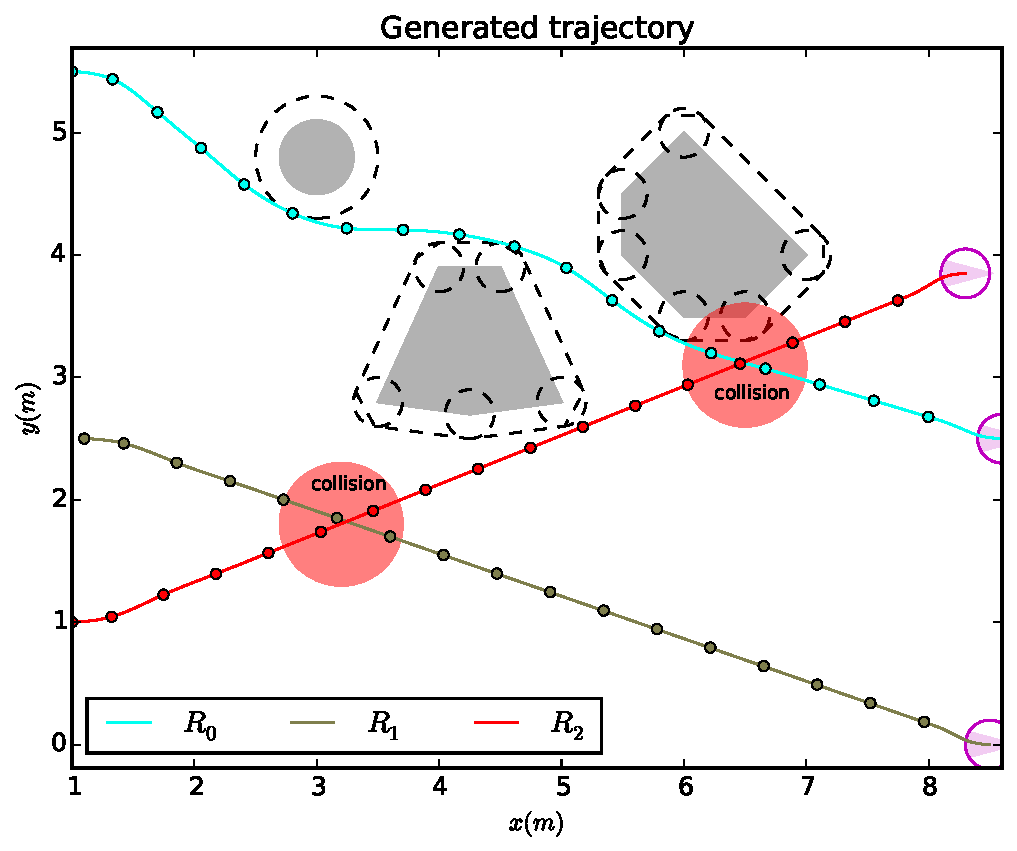
\includegraphics[width=\linewidth]{./images/collision/new/multirobot-path.pdf} %
  %\rule{5cm}{5cm} % <-- this is just a black box substitute for graphics
  \\[1mm]
  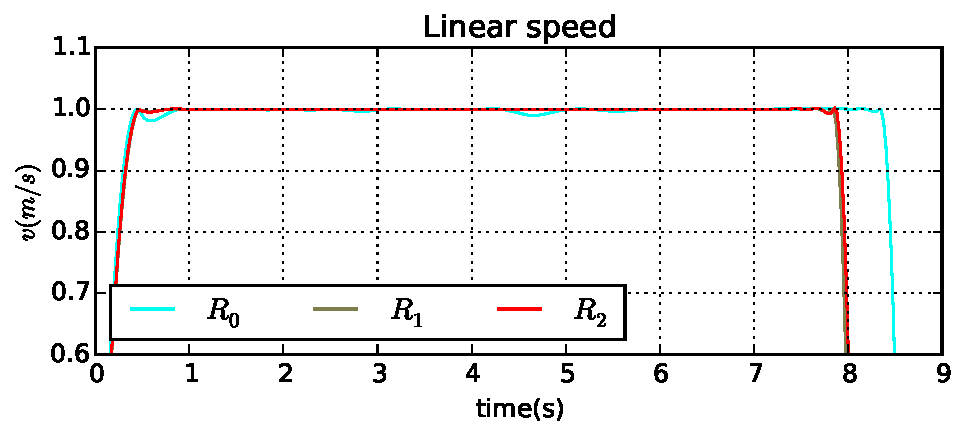
\includegraphics[width=\linewidth]{./images/collision/new/multirobot-vw.pdf} % 
  %\rule{5cm}{5cm} % <-- this is just a black box substitute for graphics
  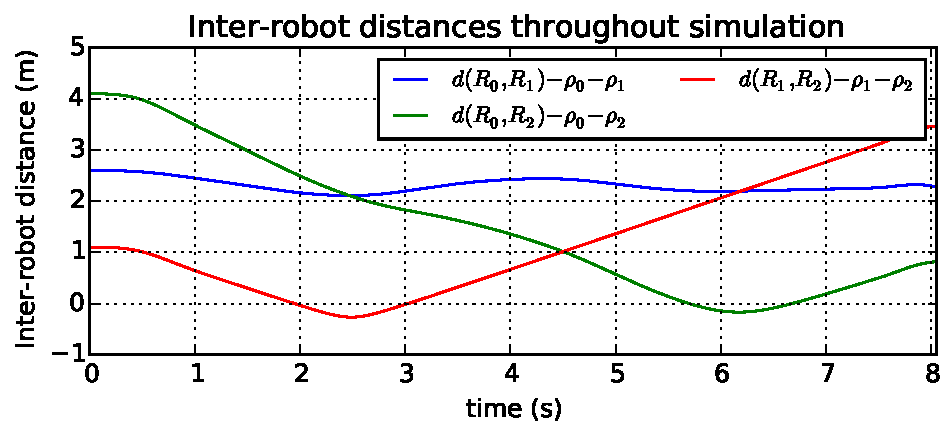
\includegraphics[width=\linewidth]{./images/collision/new/multirobot-interr.pdf} % 
  %\rule{5cm}{5cm} % <-- this is just a black box substitute for graphics
  \caption{Motion planning solution without collision handling\label{fig:collision}}
\label{fig:res}
\end{figure}

\begin{figure}\centering
  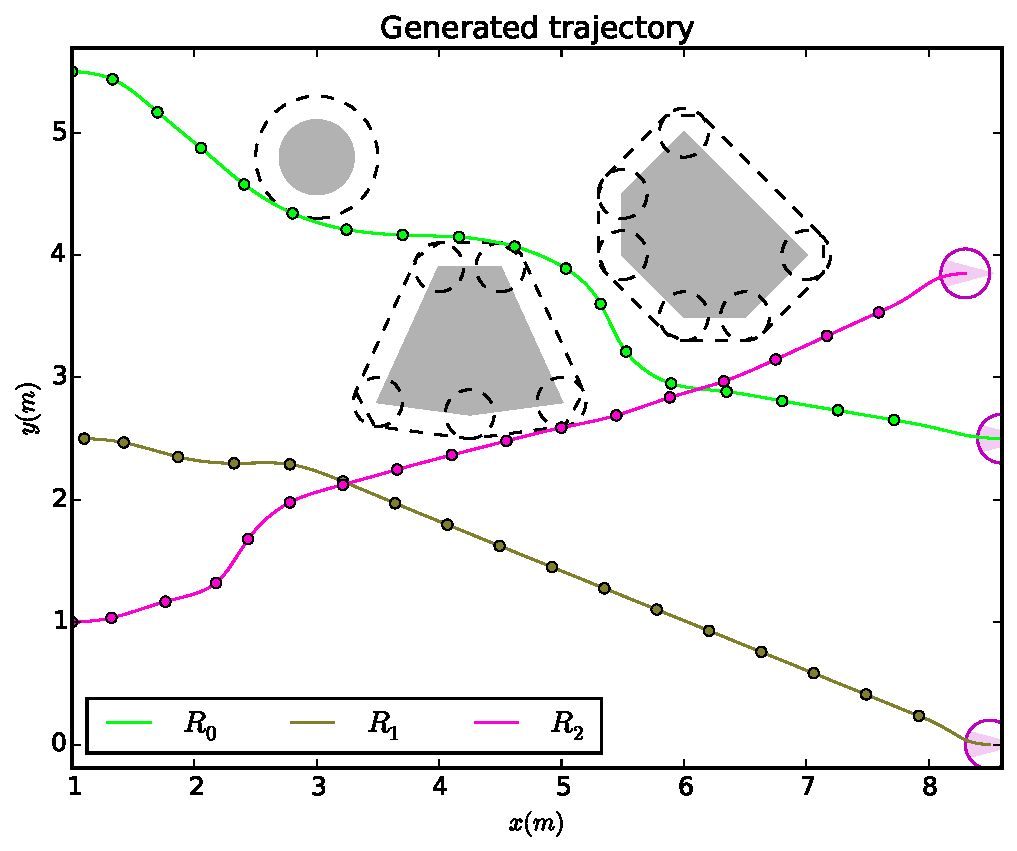
\includegraphics[width=\linewidth]{./images/no_collision/new/multirobot-path.pdf} 
% <-- use this for your graphics
  %\rule{5cm}{5cm} % <-- this is just a black box substitute for graphics
  \\[1mm]
  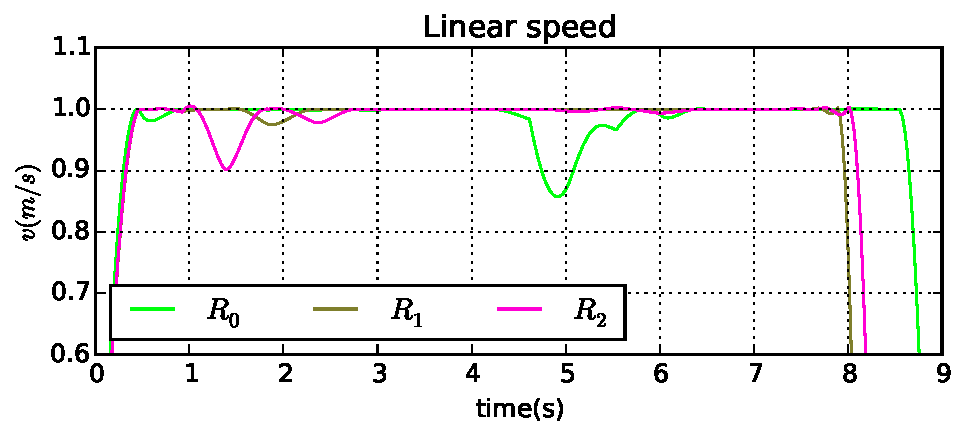
\includegraphics[width=\linewidth]{./images/no_collision/new/multirobot-vw.pdf} %
  %\rule{5cm}{5cm} % <-- this is just a black box substitute for graphics
  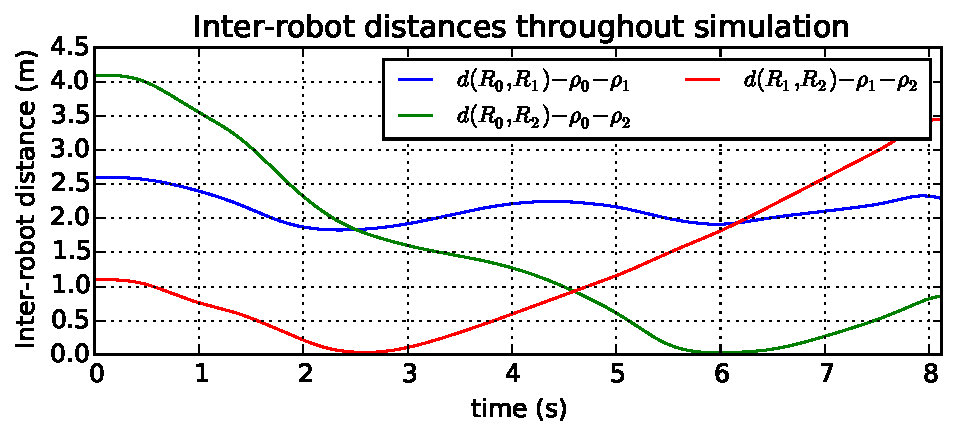
\includegraphics[width=\linewidth]{./images/no_collision/new/multirobot-interr.pdf} %
  %\rule{5cm}{5cm} % <-- this is just a black box substitute for graphics
  \caption{Motion planning solution with collision handling\label{fig:nocollision}}
\label{fig:res}
\end{figure}

For performing these two previous simulations, a reasonable number of parameters have to be set. These parameters can be categorized into two groups. \textbf{Algorithm related} parameters and the \textbf{optimization solver related} ones.
Among the former group, the most important ones are:
\begin{itemize}
\item[$\bullet$] The number of sample for time discretization ($N_s$);
\item[$\bullet$] The number of internal knots for the B-splines curves ($N_{knots}$);
\item[$\bullet$] The planning horizon for the sliding window ($T_p$);
\item[$\bullet$] The computation horizon ($T_c$).
\item[$\bullet$] The detection radius of the robot ($d_{sen}$).
\end{itemize}

The latter kind depends on the numeric optimization solver adopted.
However, since most of them are iterative methods, it is common
to have at least a maximum number of iterations and a stop condition parameters.

%The task of searching for a satisfactory set of parameters' values with regard to a performance metric (e.g. total time to complete the miss1ion) is quite laborious.

This considerable number of parameters
%having influence on the solution
%and/or on the time for finding a solution
makes the search for a
satisfactory set of parameters' values a laborious task.

Therefore, it is important to have a better understanding of how some
performance criteria are impacted by the changes in algorithm
parameters.

\subsection{Parameters' impact}

Three criteria considered important for the validation of this method were studied: {Maximum computation time} during the planning over the computation horizon ($MCT/T_c$ 
ratio); Obstacle penetration area ($P$); Travel time ($T_{tot}$).
Different parameters configuration and scenarios where tested in order to highlight
how they influence those criteria.
%We tested different parameters configuration and scenario in order to 
%understand how they influence
%those criteria.
%The three criteria defined for a given robot $R_b$ are:
%
%\begin{itemize}
%
%\item
%\textit{Maximum computation time} during the planning over the computation horizon ($MCT/T_c$ 
%ratio).
%
%\item
%Obstacle penetration area ($P$).
%
%\item
%Travel time ($T_{tot}$).
%
%\end{itemize}

\subsubsection{Maximum computation time over computation horizon $MCT/T_c$}

The significance of this criterion lays in the need of assuring the 
real-time property of this algorithm.
In a real implementation of this approach the computation horizon would have 
always to be superior than the
maximum time took for computing a plan.

%Several simulations for different scenarios with different sets of parameters were
%performed.

%For instance,
Table~\ref{tab:s3param} summarizes one of the scenarios studied for a 
single robot. Results obtained from simulations in 
that scenario are presented in Figure~\ref{fig:uni3}, for different parameters set.

Each dot along the curves corresponds to the average of $MCT/T_c$ along different $T_p$'s for a given value of ($T_c/T_p$, $N_s$).
The absolute values observed in the charts depend on the processing speed of the machine
where the algorithm is run. Those simulations were run on an Intel Xeon CPU 2.53GHz processor.

Rather than observing the absolute values, it is interesting to analyze the impact of 
changes in the parameters values. In particular, an increasing number of $N_s$ 
increases $MCT/T_c$ for a 
given $T_c/T_p$. Similarly, an increasing of $MCT/T_c$ as the number of
internal knots $N_{knots}$ increases from charts \ref{fig:uni34} to \ref{fig:uni36} is 
noticed.

Further analyses of those data show that finding the solution using the SLSPQ method
requires $O(N_{knots}^3)$ and $O(N_s)$ time. Although augmenting $N_{knots}$ can yield
to an impractical computation time, typical $N_{knots}$ values did not need to exceed $10$ in our simulations, which is a sufficiently small value.

% a greater impact of the number of samples (Ns ) and number of
%non-null internal knots (Nknots ) is observed. The greater the Nknots or the Ns the 
%greater
%is the maximum computation time /Tc . This behavior is the one expected since the 
%number
%of constraints and the number of arguments for the cost function to be minimized depend
%on these two parameters respectively.
\begin{table}[H]
\caption {Values for scenario definition} \label{tab:s3param}
\begin{center}
\begin{tabular}{c|c}
%\hline
$v_{max}$ & $1.00\ \mathrm{m/s}$\\[4pt]
%\hline
$\omega_{max}$ & $5.00\ \mathrm{rad/s}$\\[4pt]
%\hline
$q_{inital}$ & $[-0.05\ 0.00\ \pi/2]^T$\\[4pt]
%\hline
$q_{final}$ & $[0.10\ 7.00\ \pi/2]^T$\\[4pt]
%\hline
$u_{initial}$ & $[0.00\ 0.00]^T$\\[4pt]
%\hline
$u_{goal}$ & $[0.00\ 0.00]^T$\\[4pt]
%\hline
$O_0$ & $[0.55\ 1.91\ 0.31]$\\[4pt]
%\hline
$O_1$ & $[-0.08\ 3.65\ 0.32]$\\[4pt]
%\hline	
$O_2$ & $[0.38\ 4.65\ 0.16]$
%\hline
\end{tabular}
\end{center}
\end{table}
\begin{figure}[!h]
        \centering
        ~ %add desired spacing between images, e. g. ~, \quad, \qquad, \hfill etc.
          %(or a blank line to force the subfigure onto a new line)
        \begin{subfigure}[b]{0.48\textwidth}
                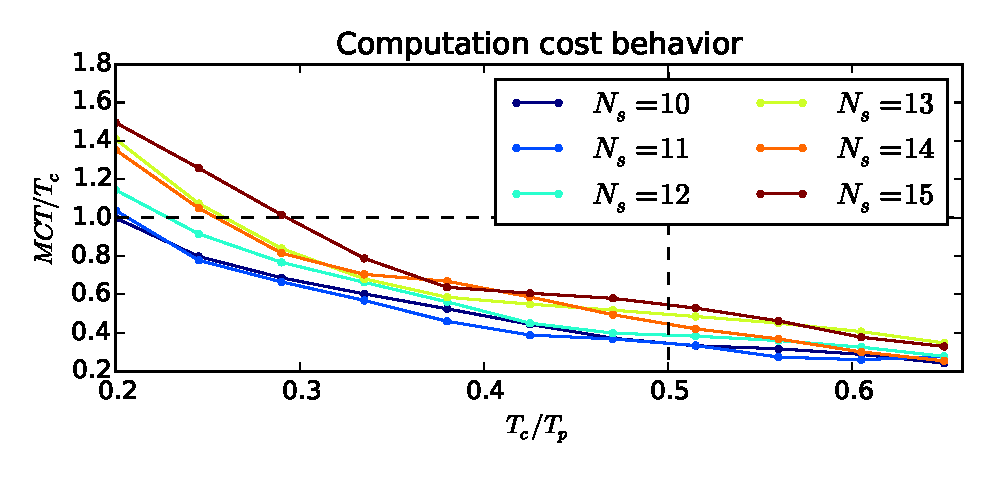
\includegraphics[width=\textwidth]{./images/realtime/Scenario_3__N_knots_4/mcttc-tctp.eps}
                \caption{Four internal knots
                %. Average variance between lines is $1.047\times 10^{-2}$
                }\label{fig:uni34}
        \end{subfigure}
        
        ~ %add desired spacing between images, e. g. ~, \quad, \qquad, \hfill etc.
          %(or a blank line to force the subfigure onto a new line)
        \begin{subfigure}[b]{0.48\textwidth}
                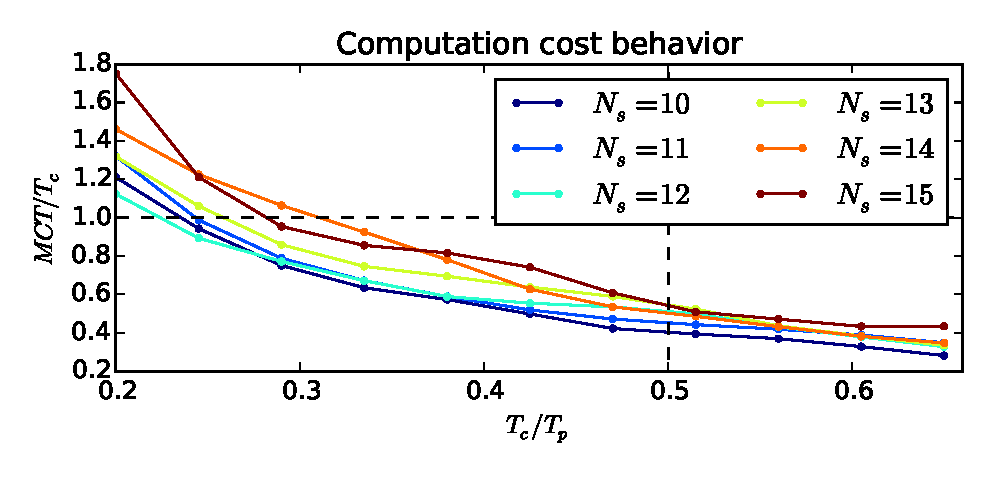
\includegraphics[width=\textwidth]{./images/realtime/Scenario_3__N_knots_5/mcttc-tctp.eps}
                \caption{Five internal knots
                %. Average variance between lines is $0.972\times 10^{-2}$
                }\label{fig:uni35}
        \end{subfigure}
        ~ %add desired spacing between images, e. g. ~, \quad, \qquad, \hfill etc.
          %(or a blank line to force the subfigure onto a new line)
        \begin{subfigure}[b]{0.48\textwidth}
                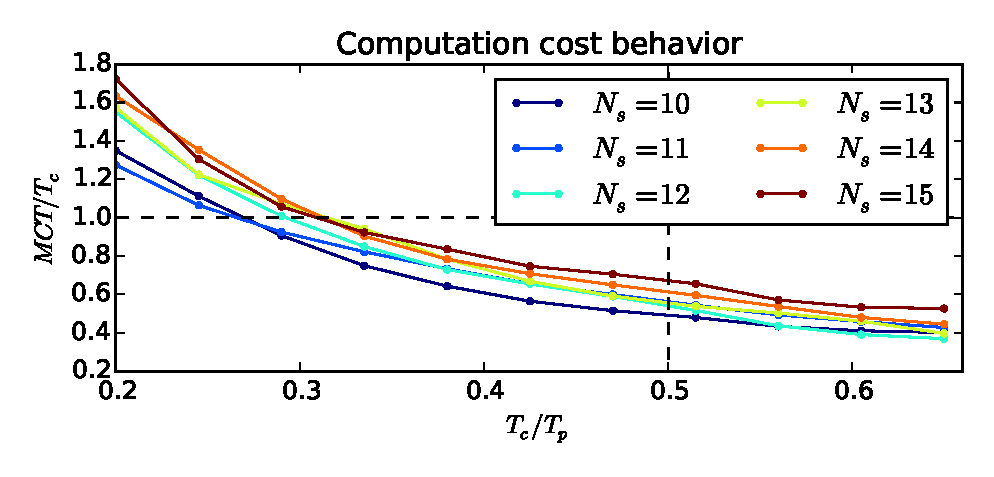
\includegraphics[width=\textwidth]{./images/realtime/Scenario_3__N_knots_6/mcttc-tctp.eps}
                \caption{Six internal knots
                %. Average variance between lines is $0.587\times 10^{-2}$
                }\label{fig:uni36}
        \end{subfigure}
        \caption{Three obstacles scenario simulations}\label{fig:uni3}
\end{figure}

\begin{figure}[!h]\centering
  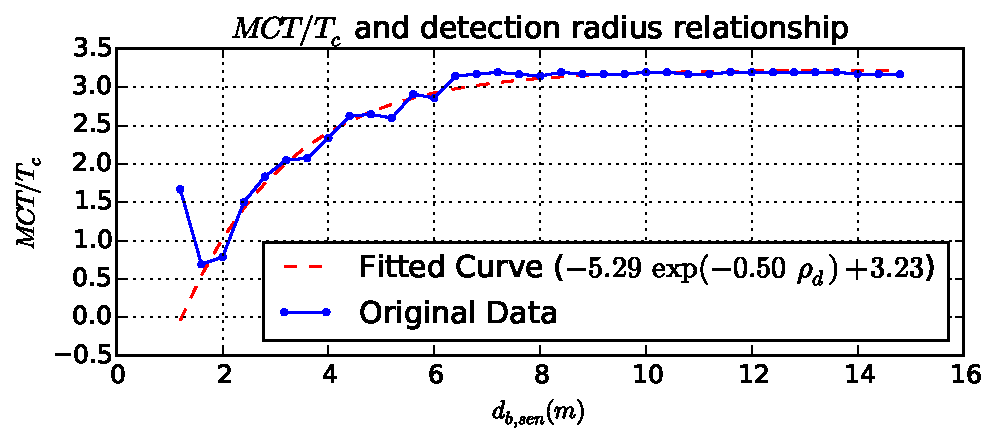
\includegraphics[width=\linewidth]{./images/drho/drho-rmp.pdf} % <-- use this
  %\rule{5cm}{5cm} % <-- this is just a black box substitute for graphics
  \caption{Increasing of detection radius and impact on a $MTC/T_c$ 
ratio\label{fig:drhormp}}
\end{figure}
Another parameter having direct impact on the $MCT/T_c$ ratio is the detection radius
of the robot's sensors.
As the detection radius of the robot increases, more obstacles are
seen at once which, in turn,
increases the number of constraints in the optimization problems.
The impact of increasing the detection radius $d_{sen}$ in the $MCT/T_c$ ratio can
be seen in Figure~\ref{fig:drhormp} for a scenario with seven obstacles.
The computation time stops increasing as soon as the robot sees all obstacles present in the environment.

%\subsection{Parameters' impact analyses}

%\begin{itemize}
% \item 
% $O(N_{knots}^3)$ time is requested; 
% \item 
% $O(N_s)$ time is requested;
%\end{itemize}

\subsubsection{Obstacle penetration $P$}

Obstacle penetration area $P$ gives a metric for obstacle avoidance and 
consequently for the solution quality. A solution where the planned trajectory does not pass through 
an object at any instant of time gives $P = 0$. The solution quality decrease with increasing P. 
However, since time sampling is performed during the optimization, $P$ is usually greater than 
zero.
A way of assuring $P = 0$ would  be to increase the obstacles radius computed by the robot's 
perception system by the 
maximum distance that the robot can run within the time spam $T_p/N_s$. However simple,
this approach represents a loss of optimality and is not considered in this work.

It is relevant then to observe the impact of the algorithm parameters in the obstacle 
penetration area.
$T_c/T_p$ ratio, $N_{knots}$ and $d_{sen}$ impact on this criteria is only 
significant for degraded cases, meaning that around typical values those parameters 
do not change $P$ significantly. However, time sampling $N_s$ is a relevant parameter.
Figure~\ref{fig:res} shows the penetration area decreasing as the number of samples 
increases.
\begin{figure}[!h]\centering
  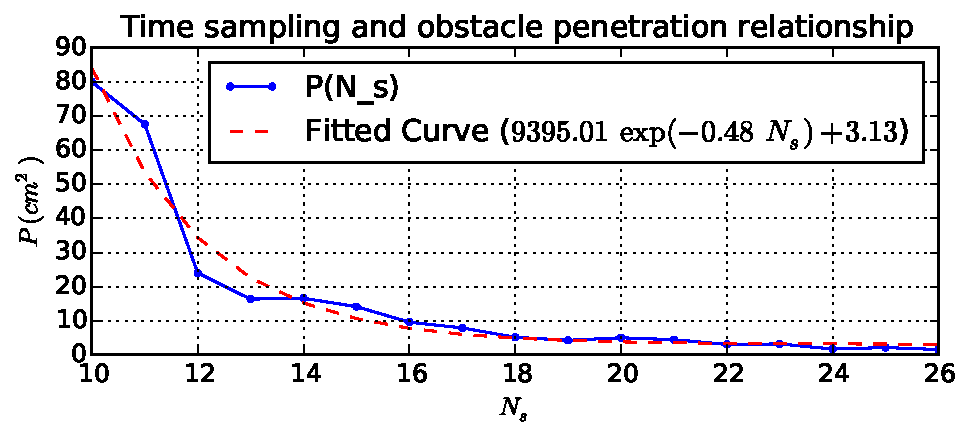
\includegraphics[width=\linewidth]{./images/penetration/pen-nsi.pdf} %
  %\rule{5cm}{5cm} % <-- this is just a black box substitute for graphics
  \caption{Obstacle penetration decreasing as sampling increases}
\label{fig:res}
\end{figure}
%\subsubsection{Detection radius impact}
%Ideally we would have Pw = 0. A way of guarantying that would be to increase the
%obstacles radius computed by the robot's perception system by the maximum distance that
%the robot can run within the time spam Tp /Ns (equivalent to Tc /NTc ). However simple,
%this approach represents a loss of optimality and will not be considered in this work.1
%These two behaviors indicate how a compromise between computation time and optimality must be found.
\subsubsection{Travel time $T_{tot}$}
%
Another complementary metric for characterizing solution quality is the travel time
$T_{tot}$. Analyses of data from several simulations show a tendency that for a given value 
of $N_{knots}$, $N_s$ and $T_c$ the travel time decreases as the planning horizon $T_p$ decreases.
This can be explained by the simple fact that for a given $T_c$, a more optimal solution (in terms of travel time) can be found if the planning horizon $T_p$ is smaller.
%Figure~\ref{fig:ttot} show data that supports these analysis.
%\begin{figure}[!h]
%        \centering
%        ~ %add desired spacing between images, e. g. ~, \quad, \qquad, \hfill etc.
%          %(or a blank line to force the subfigure onto a new line)
%        \begin{subfigure}[b]{0.48\textwidth}
%                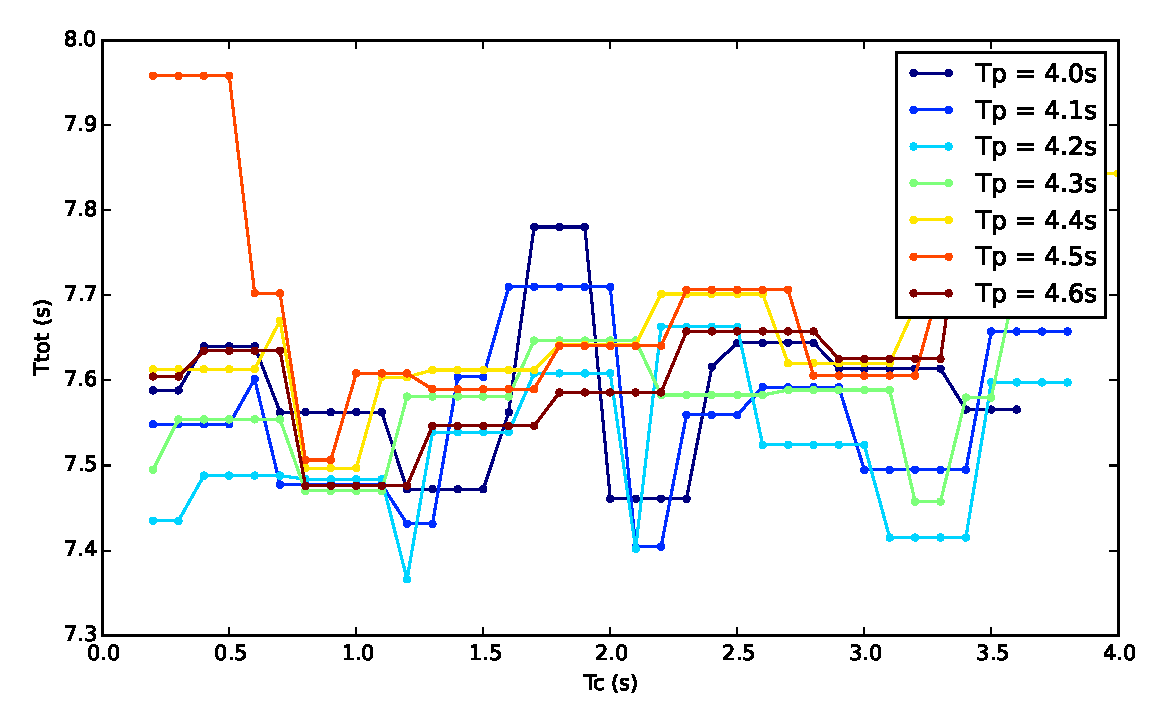
\includegraphics[width=\textwidth]{./images/tot/tot10.eps}
%                \caption{$N_s = 10$}\label{fig:ttot1}
%        \end{subfigure}
%        ~ %add desired spacing between images, e. g. ~, \quad, \qquad, \hfill etc.
%          %(or a blank line to force the subfigure onto a new line)
%        \begin{subfigure}[b]{0.48\textwidth}
%                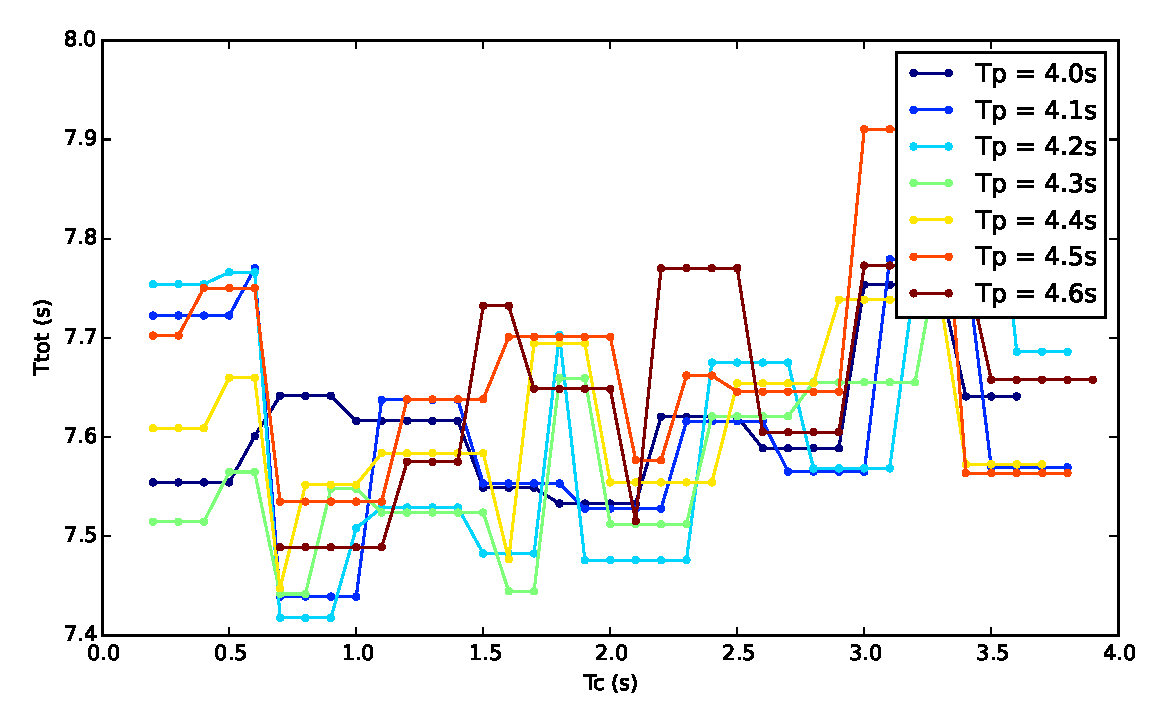
\includegraphics[width=\textwidth]{./images/tot/tot11.eps}
%                \caption{$N_s = 11$}\label{fig:ttot2}
%        \end{subfigure}
%        
%        ~ %add desired spacing between images, e. g. ~, \quad, \qquad, \hfill etc.
%          %(or a blank line to force the subfigure onto a new line)
%        \begin{subfigure}[b]{0.48\textwidth}
%                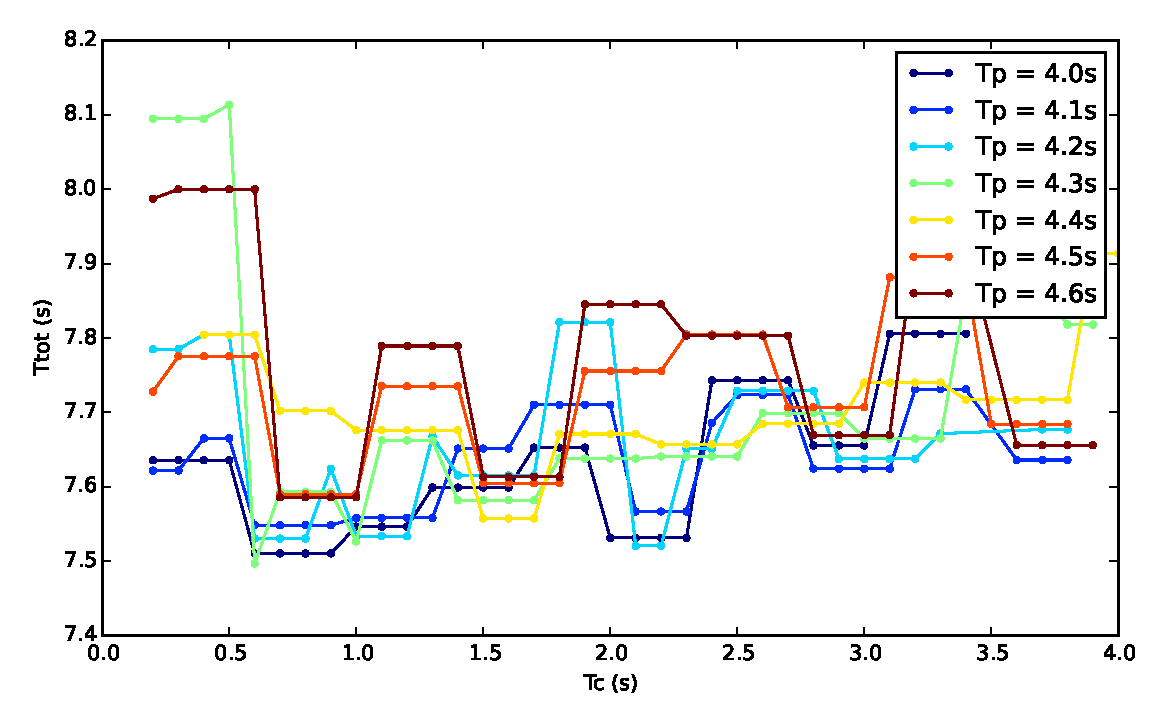
\includegraphics[width=\textwidth]{./images/tot/tot12.eps}
%                \caption{$N_s = 12$}\label{fig:ttot3}
%        \end{subfigure}
%        \caption{Variation of total travel time with the computation horizon ($T_c$) for differet planning horizons ($T_p$) and sampling number ($N_s$) in three obstacles scenarion.}\label{fig:ttot}
%\end{figure}
Another relevant observation is that the overall travel time is shorter for smaller $N_s$'s. 
This misleading improvement does take into account the fact 
that the fewer the samples the greater will be the obstacle penetration area as shown previously in Figure~\ref{fig:res}.

Furthermore, Figure~\ref{fig:drhotot} shows travel time
invariance for changes in the detection radius far from degraded values that are too small.
This points out that a local knowledge of the environment provides enough information for finding good solutions.
\begin{figure}[!h]\centering
  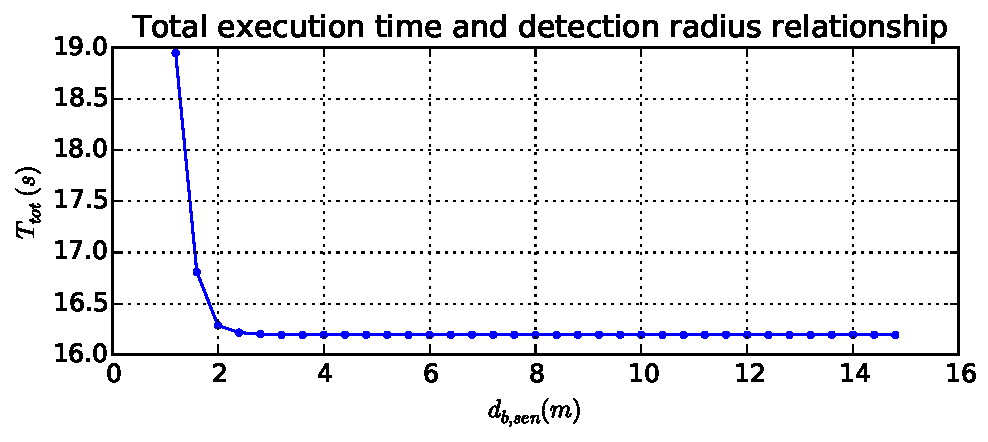
\includegraphics[width=\linewidth]{./images/drho/drho-tot.pdf}
  \caption{Increasing of detection radius and impact on
  $T_{tot}$\label{fig:drhotot}}
\end{figure}

%Valid for SLSQP-based sovler:
%
%\begin{itemize}
% \item [$\bullet$] $MCT/T_c$ is $O(n^3)$ time dependent where $n$ is directly proportional to $N_{knots}$;
% \item [$\bullet$] $MCT/T_c$ is $O(n)$ where $n$ is directly proportional to $N_s$;
% \item [$\bullet$] $MCT/T_c$ increases as the detection radius of the robot increases;
% \item [$\bullet$] $T_{tot}$ decreases as $N_s$ decreases (up to a minimum value);
% \item [$\bullet$] $T_{tot}$ is not influenced by $T_c$ in a observable way;
% \item [$\bullet$] $T_{tot}$ decreases as the $N_{knots}$ increases (but not indefitalely);
% \item [$\bullet$] $P$ increases as $N_s$ decreases (up to a maximum value);
%\end{itemize}
%
%"Semantic" interpretation/analysis of the obstacles can speedup NPL solving by reducing the number of contraints.
%
%"Calibration" of the parameters can be done once knowing the real application conditions:
%\begin{itemize}
% \item [$\bullet$] Approx. obstacles "density";
% \item [$\bullet$] Robots max speed;
% \item [$\bullet$] Approx. distance;
% \item [$\bullet$] etc.
% \end{itemize}
%by simulating before and pay attention to the behavior of important values such as $MCT/T$, $T_{tot}$, $P$.



%TODO Comparison with the other method;
%
%TODO Before concluding do comparison with other approach and make sure to have 
%multi-robot stuff

\section{Conclusions}

A distributed motion planner based on a receding horizon approach, modified for taking into account 
termination constraints, was proposed. Near the goal configuration 
neighborhood, the receding horizon approach is finished and a termination planning 
problem is solved for bringing the robots to their precise final state.
The problem is stated as a constrained optimization problem. It minimizes the time 
for reaching a goal configuration through a collision-free trajectory securing communication between robots. Circle and convex polygon representation of obstacles are supported.
Key techniques for implementing the motion planner are: system flatness property, 
B-spline parameterization of the flat output and SLSQP optimizer.
Finally, solutions using this planner for different scenarios were generated in 
order to validate the method. Impact of different parameters on 
computation time and quality of the solution was analyzed.
Future work will be performed in physics simulation environment where dynamics is taken into account as well as sensors models and communication latency.


%\begin{nomenclature}
%\item[kg\,m^-3]{\varrho}{Liquid density}
%\item[Pa]{p}{Liquid pressure}
%\medskip
%\item{\mathit{Re}}{Reynold's number}

%\begin{acknowledgements}
%G.~Surname was supported by grant 1234567890.
%\end{acknowledgements}

%TODO perspectives
%
%Analise influence of dynamics of system, sensors, communication latency;

%\newpage
%\mbox{}\newpage

\bibliographystyle{actapoly}
\bibliography{biblio}

\end{document}
%kate: default-dictionary en;